\documentclass[10pt]{article}

% Lines beginning with the percent sign are comments
% This file has been commented to help you understand more about LaTeX

% DO NOT EDIT THE LINES BETWEEN THE TWO LONG HORIZONTAL LINES

%---------------------------------------------------------------------------------------------------------

% Packages add extra functionality.
\usepackage{
	times,
	graphicx,
	epstopdf,
	fancyhdr,
	amsfonts,
	amsthm,
	amsmath,
	algorithm,
	algorithmic,
	xspace,
	hyperref}
\usepackage[left=1in,top=1in,right=1in,bottom=1in]{geometry}
\usepackage{sect sty}	%For centering section headings
\usepackage{enumerate}	%Allows more labeling options for enumerate environments 
\usepackage{epsfig}
\usepackage[space]{grffile}
\usepackage{booktabs}
\usepackage{amsmath}
\usepackage[super]{nth}
\usepackage{array}

% This will set LaTeX to look for figures in the same directory as the .tex file
\graphicspath{.} % The dot means current directory.

\pagestyle{fancy}

\lhead{\YOURID}
\chead{\MyLang: Language Specification}
\rhead{\today}
\lfoot{CSCI 334: Principles of Programming Languages}
\cfoot{\thepage}
\rfoot{Spring 2022}

% Some commands for changing header and footer format
\renewcommand{\headrulewidth}{0.4pt}
\renewcommand{\headwidth}{\textwidth}
\renewcommand{\footrulewidth}{0.4pt}

% These let you use common environments
\newtheorem{claim}{Claim}
\newtheorem{definition}{Definition}
\newtheorem{theorem}{Theorem}
\newtheorem{lemma}{Lemma}
\newtheorem{observation}{Observation}
\newtheorem{question}{Question}

\setlength{\parindent}{3pt}

%---------------------------------------------------------------------------------------------------------

% DON'T CHANGE ANYTHING ABOVE HERE

% Edit below as instructed
\newcommand{\MyLang}{My Mandala Image Generataion}	% Replace MyLang with your language name #
\newcommand{\PartnerOne}{Kelly M.}	% Replace PartnerOne with your name #
\newcommand{\PartnerTwo}{Lauren M.}	% Replace PartnerTwo with your partner's name #
\newcommand{\YOURID}{\PartnerOne{} + \PartnerTwo{}} % Remove \PartnerTwo if working alone.


\title{\MyLang: Language Specification}
\date{Spring 2022}
\author{\PartnerOne{} and \PartnerTwo{}} % Remove \PartnerTwo if working alone.

\begin{document}
\maketitle

\vspace{\baselineskip}	% Add some vertical space

% Refer to the lab handouts to determine what should go in each of these sections.  Each lab is additive.  So lab 8 should include everything you wrote in lab 7.  Lab 9 should include everything you wrote in lab 8, etc.

\section{Introduction}

The problem that our language solves is image generation for mindfulness-based
practices. When we started brainstorming ideas we thought: what comes to mind
when people think of the field of "computer science"? Truthfully, we feel that
computer science can have very rigid, stereotypical associations. On a surface
level, many may think that the purpose of computer scientists is to only develop
applications or provide the underlying code that allows electronic devices to run.
While these are true, we want to push the bounds of who and what the field of computer
science can be for. The two of use, being college students ourselves, have
definitely had our fair share of experiences with gumption traps, frustrations,
self-doubt and the imposter syndrome in our time in CS. We asked ourselves:
how can we design a language that is removes the nervousness or stereotypes from
computer science? We began to think of the recent push for mental health advocacy
and specifically the utilization of mindfulness-based practices to regulate
depression and anxiety. Given the examples we were shown in class that involved
pattern and image generation, we began to consider the possibility of Mandala
coloring pages.
  \\\\This problem needs its own programming language because it offers a wide array
of engagement levels for users. For the user who simply wants to generate a
personal Mandala coloring page, they can do so quickly and with little engagement
with the code. For the user who wants to be introduced to the underlying code of the programming
language, we allow them to write more code-specific preferences. We hope to gradually
introduce coding specifications to users while also giving them an end-product that
will hopefully aid with emotion regulation. We think this is a great opportunity
to engage another discipline in our CS work.

		
\section{Design Principles}

The foundational principles that underpin our language are 
simplicity and accessibility. We intend for these two descriptors 
to reinforce each other. We strive to offer our users a simple 
interface to work with that simultaneously generates beautiful 
Mandala design patterns. The accessibility component of our language 
refers to the varying levels of engagement that a user can take part in. 
We want to allow users who are completely new to coding to be able to 
provide an extent of personalization in their designs while hiding some 
of the underlying implementation. However, for a more technically-experienced 
user, we want to unveil some of the backend coding that generates the Manala images. 
In this way, we hope to make possible different levels of design intricacy and 
detail that promotes a flexible interface, allowing the user to exercise creativity.

\pagebreak[4]

\section{Example Programs}

    \textbf{Example 1: Level I Mandala}
    
	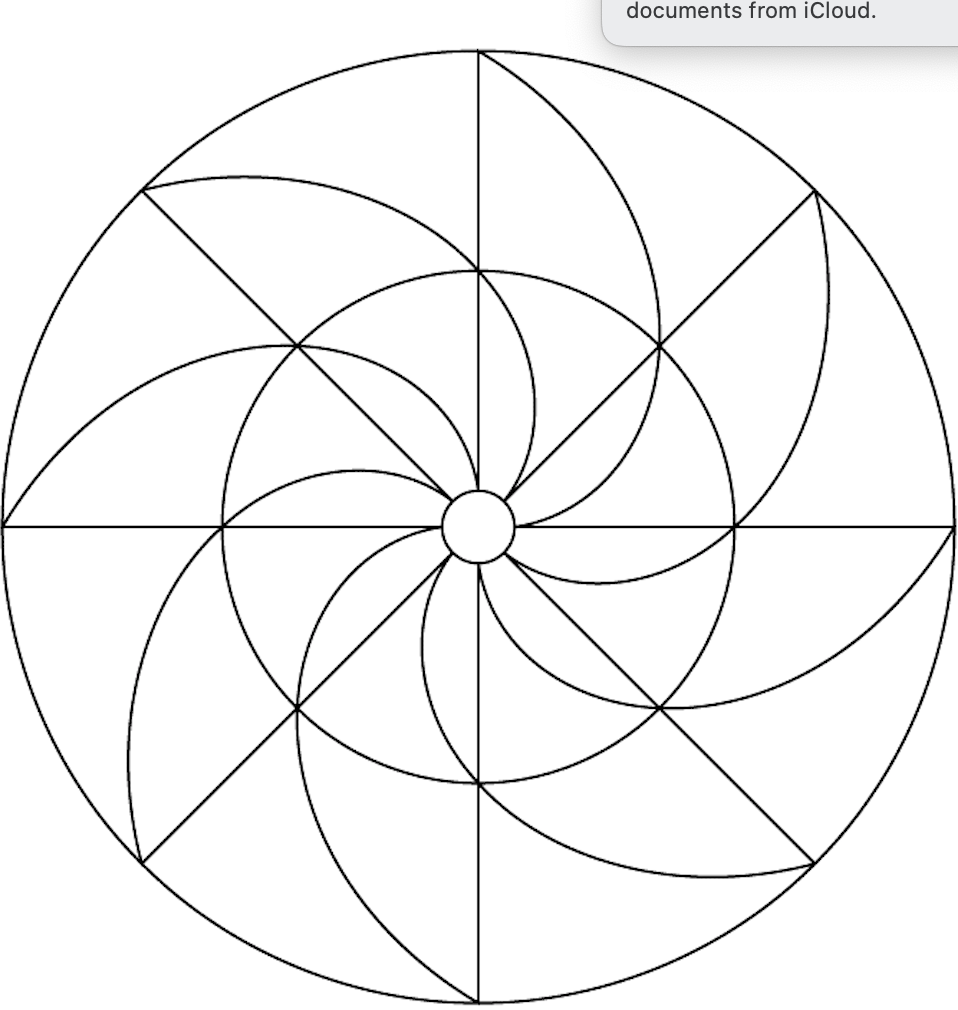
\includegraphics[width=0.45\textwidth]{images/examp1outline.jpg}
	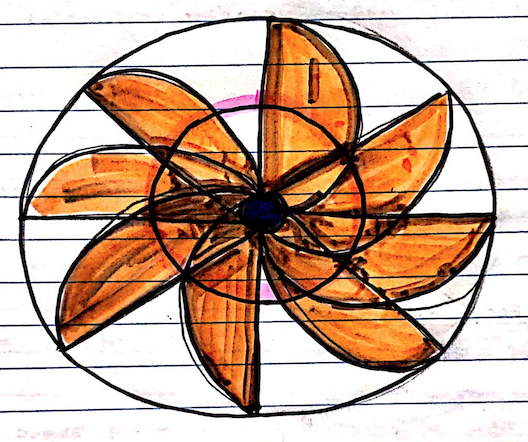
\includegraphics[width=0.45\textwidth]{images/examp1.jpg}

	\textit{*Apologies, the black marker bled a little bit in the middle of the drawing}
	\\\textbf{Code:}

	\begin{verbatim}

inner_circle = (circle, area = 2, outline_col=“black”, fill_col =“blue”)
second_circle = (circle, area = 6, outline_col=“black”, fill_col =“white”)
outer_circle = (circle, area = 12, outline_col=“black”, fill_col= “white”)

petals = 
	petal_1 = (half_leaf, half_leaf_width = 3, start = (inner_circle+12))
	petal_2 = rotate(petal_1, start = 45)
	petal_3 = rotate(petal_2, start = 45)
	…
	petal_8 = rotate(petal_7, start = 45)

stop := when rotate value = 360

\end{verbatim}

\pagebreak[4]

\textbf{Example 2: Level II Mandala}
    
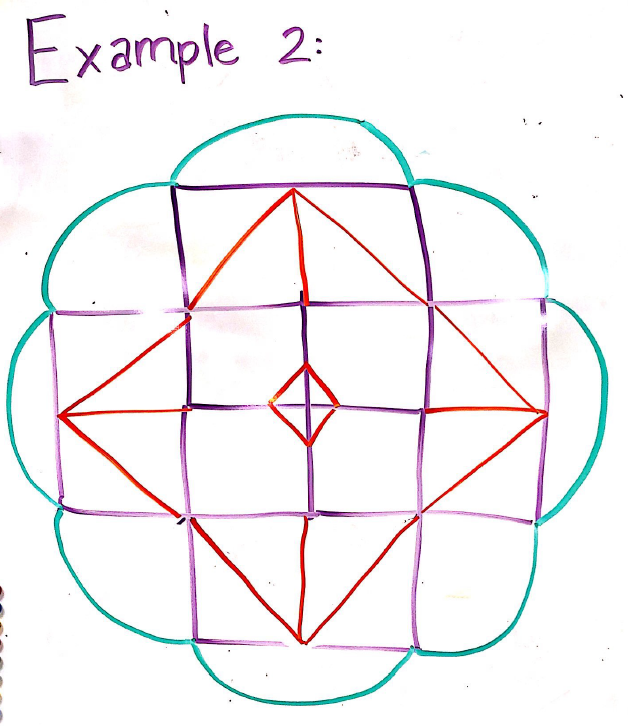
\includegraphics[width=0.45\textwidth]{images/example2.jpg}

\begin{verbatim}

	center = (rhombus, dimensions(1, 2), outline_col="orange", fill_col="white")

	begin turtle at center of center shape(rhombus)
		turtle.col="purple"
		(1) Move turtle left by 2.5 pts., up 5, over 5, down 5, over 2.5
		(2) repeat 4x for each of the four overlapped purple squares

	begin turtle at center of center shape(rhombus)
		turtle.col="orange"
		(1) Move turtle up by 5 (without beginning trace yet)
		(2) Put turtle down (to begin trace)
		(3) Rotate turtle 45 degr. and draw diagonal
			(a) stop turtle after 7 paces (length of the diagonal of
			one of the trianlges is ~3.5 so 2*3.5 = 7)
		(4) Repeat 4x until turtle back at beginning

	begin turtle at center of center shape(rhombus)
		turtle.col="green"
		turtle = (semicircle, radius=3, col="green") //specify the intended shape 
		we want to create with the turtle
		(1) Move turtle left 2.5, up 5
		(2) Begin semicircle drawings, rotate by ~30 degrees after compelting each
		(3) Repeat 8x until turtle back at beginning
	
\end{verbatim}
	
\pagebreak[4]

\textbf{Example 3: Level II Circular Mandala}
    
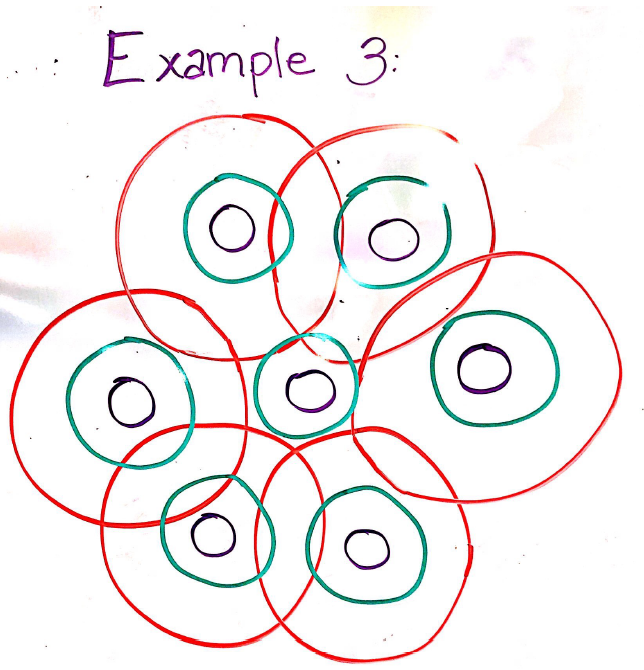
\includegraphics[width=0.45\textwidth]{images/example3.jpg}

\begin{verbatim}

	Pattern: 

	inner_circle = (circle, area = 2, outline_col=“purple”, fill_col =“white”)
	middle_circle = (circle, area = 6, outline_col=“green”, fill_col =“white”)
	outer_circle = (circle, area = 12, outline_col=“red”, fill_col= “white”)
	
	Center: 
	center = (circle, area = 2, outline_col="purple", fill_col="white")
	center_outline = (center + (radius = 1, ouline_col="green")

	(1)  Construct center
	(2)  (turtle is currently pointed upwards in resting position)
		(a) Rotate turtle 45 degr. and move by 5 pts.
	(3) Implement specified pattern above via the turtle
	(4) Repeat 6x
	
	* Note: in this particular implementation, rather than remaking each
	shape for each iteration, we developed a general Pattern that is made up of three
	distinct parts (a small, medium-sized, and large circle). In our beginning
	stages of this design process, we are beginning to consider how 'Patterns'
	can operate similarly to classes in the Java language and in order to reuse
	the patterns, we just create a new instance of the class. 
	
	\end{verbatim}

\section{Language Concepts}

We plan to define the “primitives” of our languages as being simple shapes, lines, 
or other small details that make up larger geometric shapes. In terms of “combining 
forms,” it is our goal to have the user consider how the geometric shapes of our 
designs are built in relation to one another. For example, in the first example up
above, we can see the intricacies of a larger design. However, as we break it down 
in our mind’s eye, we can see that at the base level, it is really made up of three 
different circles (one small, medium, and one large). The circles are placed at 
proportional distances to one another. The outer circle is broken into four quadrants. 
From there, we can envision how a ‘turtle’ (a point or marker in our program) can begin
 in one location of our design and work its way outwards until eventually returning to 
 the beginning. The recursive nature of our language is one of its beautiful features.

\section{Syntax}

The overarching component of our language: The Mandala Image.

\begin{verbatim}

	<shape> := <circle> <square> <rectangle>< isosceles triangle> <rhombus> <line>
	<color> := <red> <orange> <yellow> <green> <blue> <purple>
	<radius> := n in range(1… 8)
	<dimensions> := <x in range (1…8)>< y in range(1…8)>
	<center> := <shape><radius> | <shape><dimension>

	We imagine a Java class-type implementation that will allow us to 
	build instances of and implement certain pre-defined patterns

	class Pattern
	image.shape = circle
	image.color = blue
	image.outline = black

\end{verbatim}

\section{Semantics}

\subsection{What are the primitive kinds of values in your system? For example, a primitive might be a number, 
a string, a shape, a sound, and so on. Every primitive should be an idea that a user can explicitly 
mention in a program.} 
 
The primitive values in our system are the shapes, which comprise each base layer of the larger pattern.
Another primitive is the color, used to specify both the shape and the turtle color. Another primitive
is the unit of measurement (We are considering making a fun new unit of measurement but for the time being
we are basing this project proposal off of terms of pts. or cm for measurements). The unit of measurement
primitive type will help with spacing the shapes apart as well as defining the radius of circles and 
the dimensions of shapes such as a rhombus, rectangle or square.

\subsection{What are the “actions” or compositional elements of your language? In other words, how are values combined? For example, your system might combine primitive 
“numbers” using an operation like “plus.” Or perhaps a user can arrange “notes” in a “sequence.”}

We like to consider the combining forms of our language as the layers or “layering processes.” 
Just as we would perform string concatenation, or combine sequences of numbers in a mathematical 
expression, so will we layer the primitive forms (shapes, colors and units of measurement) on top of one another to 
construct gradually more complex designs. 

\subsection{How is your program represented? In other words, what components (types) will be used 
in your AST? If it helps you to think about this using ML algebraic data types, please use them. 
Otherwise, a rough sketch like a class hierarchy drawings or even a Java class file is OK.}

First, we want to define an outer base shape (rectangle or circle). From there, we may 
decide how to divide the inner quadrants of the base shape. We can think most abstractly as the 
lagest layering being the end-product pattern. In our ASTs, we can break down this pattern into 
the elements (shapes, colors, dimensions, spacing, etc.) that make it up.

For inspiration in understanding we used these resources:
\\(i) https://fsharpforfunandprofit.com/posts/13-ways-of-looking-at-a-turtle/ 
\\(ii) https://lorgonblog.wordpress.com/2010/04/16/fun-with-turtle-graphics-in-f/
\\\\For help with understanding the hierarchies we referenced the hierarchy drawings displayed below.
Note, one of these is a general geometric shapes display and the other is represented
in the Java language. For our final implementation, our ASTs will be based off of F\# but
these images were just for preliminary brainstorming:

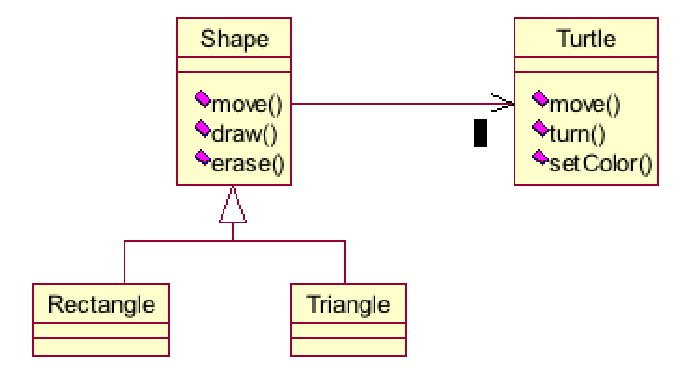
\includegraphics[width=0.45\textwidth]{images/geometric-shapes.jpg}
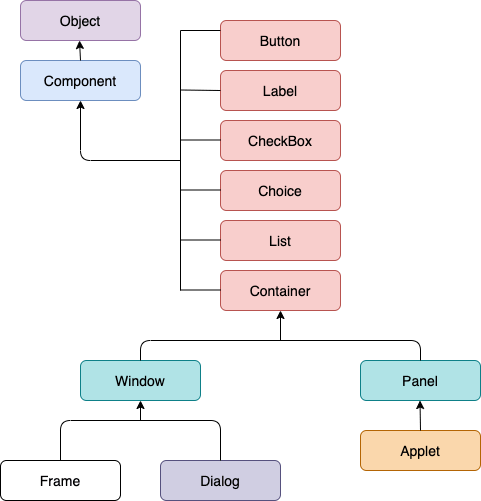
\includegraphics[width=0.45\textwidth]{images/program-in-java.png}


\subsection{How do AST elements “fit together” to represent programs as abstract syntax? For the three example 
programs you gave earlier, provide sample abstract syntax trees.}

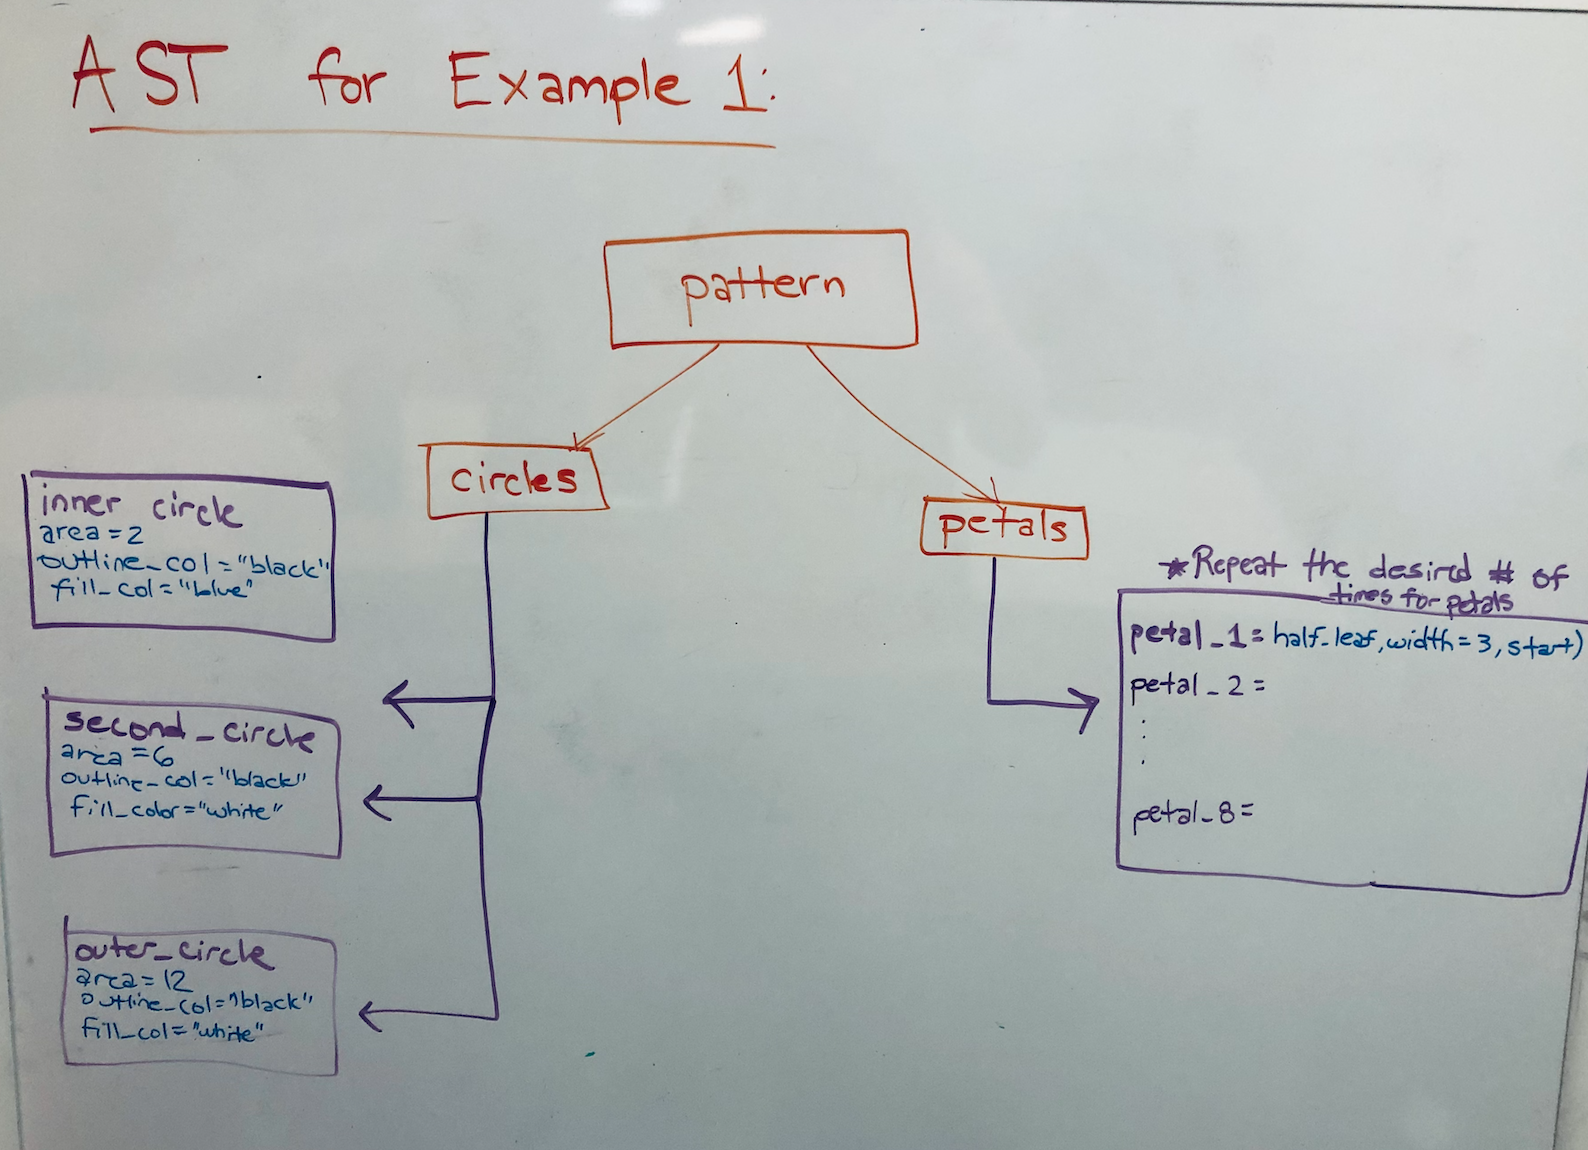
\includegraphics[width=0.75\textwidth]{images/ast1.jpg}
\\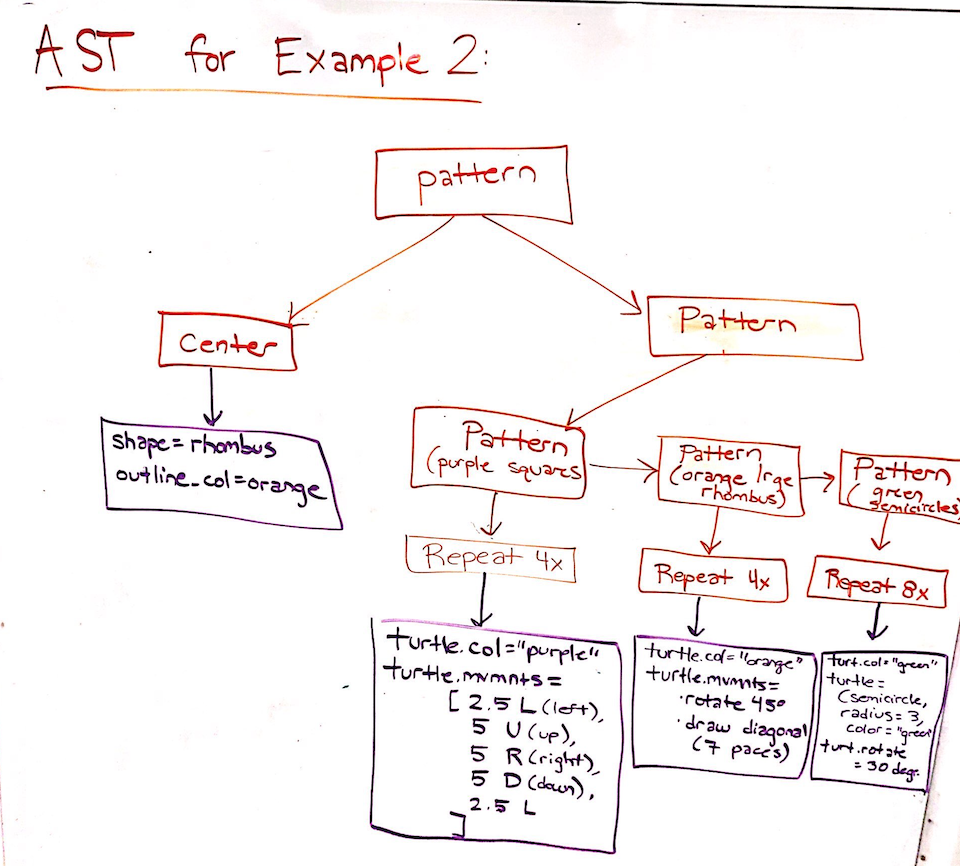
\includegraphics[width=0.75\textwidth]{images/ast2.jpg}
\\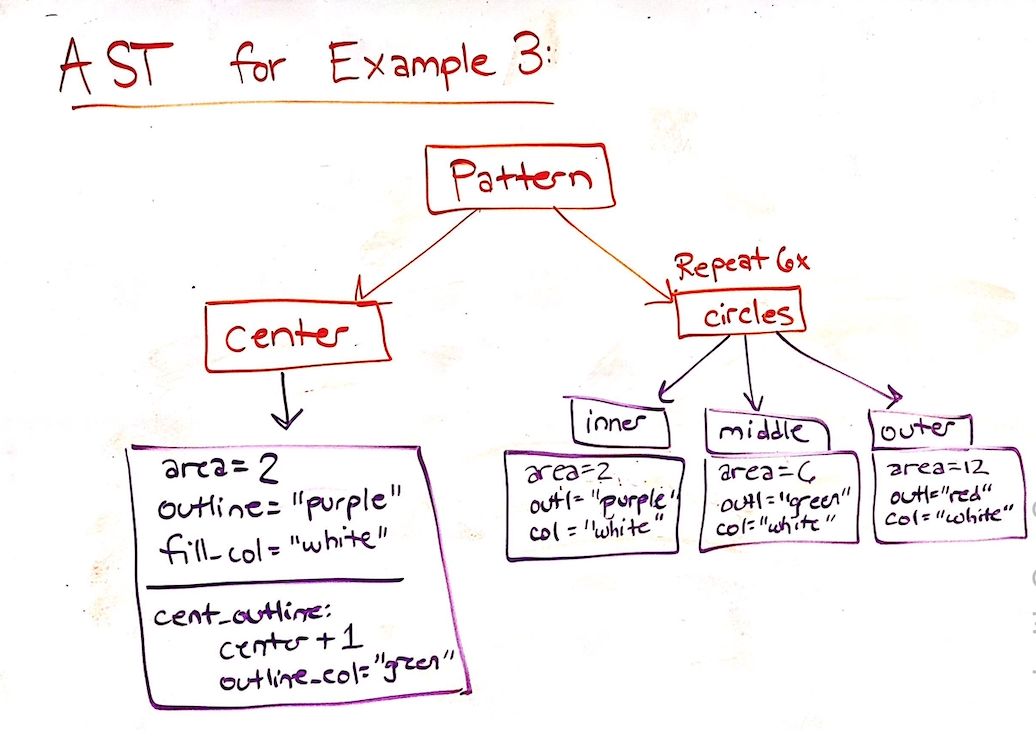
\includegraphics[width=0.75\textwidth]{images/ast3.jpg}

\subsection{How is your program evaluated? In particular, Do programs in your language read any input?
What is the effect (output) of evaluating a program? Evaluation is usually conceived of as a post-order 
traversal of an AST. Describe how such a traversal yields the effect you just described and provide 
illustrations for clarity. Demonstrate evaluation for at least one of your example programs.}

	While programs in our language do not read input explicitly from a command line, we do intend
	to implement functionality to allow the user to select from a series of drop-down menus to specify
	the specific shapes, colors or patterns that they want in their specific mandala. The output of our
	programs will be both a black outlined version of the image generated in addition to a color-filled 
	version of the mandala image. In this way, the user can print out the image and trace it out in the 
	specified colors if they so desire. Otherwise, they can just keep the already color-filled mandala image. 
	A depth-first traversal of our ASTs would be most indicative of the output of our program evaluation.
	This is because we would need to fully develop each of the specified sub-images(shapes) within the larger
	pattern before we can work our way outwards and develop other sections of the pattern. Specifically, we
	first begin by creating the center of the image and base our subsequent images off of it.
	\\\\Evaluation for Example 3 from above:

(1) Use turtle cursor to generate the center circle image (purple) and the center outline (green)
	\\(2) Create first iteration of the general Pattern (inner circle, middle circle, outer circle)
	\\(3) Hit the iteration checkpoint and repeat the general Pattern type 6 times
	\\(4) Traverse backwards to the general overall pattern at the root of the AST (representing the final mendala
	image)

\section{Minimal Formal Grammar}

% DO NOT DELETE ANYTHING BELOW THIS LINE
\end{document}